\subsection{(Anti-)(hyper-)nuclei production} 
\label{sec:nuclei}
\subsubsection{Testing thermal production and nucleon coalescence models}
\label{sec:producionmodels}

The production of light (hyper-)nuclei and their anti-matter counterparts is modeled within the scenarios of thermal-statistical hadronisation and nucleon coalescence.
In the thermal-statistical approach~\cite{Andronic:2010qu,Andronic:2017}, particles are produced from a fireball in thermal equilibrium with temperatures of the order of \Tchem~$\approx$~156~MeV that are near the temperature of the QCD phase transition boundary, as predicted by lQCD calculations \cite{Bazavov:2014pvz,Bellwied:2013cta}.
The yields of the produced objects depend on the chemical freeze-out temperature \Tchem (when inelastic collisions cease) and the mass $m$ of the object, and approximately scale as d$N$/d$y \propto \exp(-m/\Tchem)$.  
Thermal-statistical models have been successful in describing light-flavour particle production across a wide range of energies in nucleus-nucleus collisions \cite{Andronic:2017, Acharya:2017bso}.  
Due to their large mass, light (anti-)(hyper-)nuclei are particularly sensitive to \Tchem and since they are not affected by feed-down from higher mass states \cite{Andronic:2017}, the measurement of their production constitutes a precision test for the thermal model.  

In the coalescence scenario, composite objects are formed at kinetic freeze-out by coalescence of nucleons that are close in configuration and momentum space \cite{Butler:1963, Kapusta:1980, Bergstrom:1979gpv, Sato:1981ez, Nagle:1996vp, Scheibl:1998tk}. Calculations of the coalescence probability based on a density matrix approach \cite{Scheibl:1998tk} require the knowledge of the nucleus wave function and identify the volume of the particle source as the homogeneity volume that can be extracted via Hanbury-Brown-Twiss interferometry \cite{Wiedemann:1999qn}. 
The size of the (hyper-)nucleus is identified with the size parameter of its wave-function, which is related to the (measurable) rms of the charge distribution by simple relations \cite{Sato:1981ez, Bellini:2018epz}. 

While there are several theory groups working on the calculation of the expected coalescence \cite{Scheibl:1998tk, Cho:2017dcy, Zhang:2018euf, Bazak:2018hgl, Zhao:2018lyf} and thermal production rates \cite{Andronic:2010qu, Wheaton:2004qb, Petran:2013dva}, predictions reported in Fig.~\ref{fig:BAmodels} rely on the study presented in~\cite{Bellini:2018epz}, which contrasts the two production scenarios. 
In order to distinguish them, a measurement of the coalescence parameter for (anti-)(hyper-)nuclei that differ by mass, spin and size 
%(quantified by the charge rms radius or the size parameter of the wave function) 
as a function of source volume (or source radius) is proposed. 
%
The coalescence parameter \BA is defined as 
%
\begin{equation}
E_{A}\frac{\mathrm{d}^{3}N_{A}}{\mathrm{d}p_{A}^{3}}=B_{A}{\left(E_{\mathrm{p,n}}\frac{\mathrm{d}^{3}N_{\mathrm{p,n}}}{\mathrm{d}p_{\mathrm{p,n}}^{3}}\right)^{A}}\left\vert_{\vec{p}_{\mathrm{p}}=\vec{p}_{\mathrm{n}}=\frac{\vec{p}_{A}}{A}} \right.,
\label{eq:BA}
\end{equation}
%
\noindent where $p_{\mathrm{p,n}}$ are the momenta of the proton and neutron and $E_{p,n}$ their energies. In the coalescence model (black curves in top panels of Fig.~\ref{fig:BAmodels}), the coalescence parameter is determined analytically. The thermal model predicts \pT-independent particle yields at a given \Tchem, therefore a Blast-Wave (BW) model is used in \cite{Bellini:2018epz} to describe the \pT-dependence of (hyper-)nuclei and nucleon production. With the \pT~spectra of (hyper-)nuclei and protons obtained in this way, Eq.~\ref{eq:BA} is used to extract \BA (dashed blue curve in top panels of Fig.~\ref{fig:BAmodels}). 
Similarly, the coalescence parameter is obtained experimentally from Eq.~\ref{eq:BA} using the measured (hyper-)nucleus and proton \pT~distributions as input.
%
The size of the source can be sampled by means of multiplicity- and centrality-differential measurements.
%

The particle with the strongest sensitivity to the production mechanism appears to be the hypertriton (a p$\Lambda$n bound state) with its large charge rms radius of about 10 fm, for which the coalescence and the thermal model predictions differ by up to three orders of magnitude as a function of the source radius. 
While the hypertriton seems to be largely suppressed with respect to \hethree~($\mathrm{pnn}$), the \hypfour\ ($\mathrm{pp}\Lambda\mathrm{n}$) is predicted to have only a slightly lower coalescence probability with respect to \hefour~($\mathrm{ppnn}$). 
Moreover, for small $R$, i.e. in small systems as those formed in \pp and \pPb collisions, \hyp~is predicted by coalescence to be suppressed by about a factor of 100 with respect to \hethree. 
These considerations motivate systematic multi-differential measurements of \Anucl = 3 and \Anucl = 4 nuclei and hyper-nuclei as a function of multiplicity and from small (\pp, \pPb) to large systems (\PbPb) to test the validity of the coalescence picture as opposed to thermal production.

With an integrated luminosity \Lint~=~10~\nbInv in \PbPb collisions in Runs 3 and 4, \BA for \hethree, \hyp~and \hefour~can be measured in ALICE in up to ten centrality classes with a statistical precision lower than 5$\%$, 10$\%$ and 20$\%$, respectively.
The projected relative statistical uncertainties on \BA ($\sigma_{\mathrm{stat}}$/\BA) for (hyper-)nuclei with \Anucl~>~2 are reported in the central row of panels of Fig.~\ref{fig:BAmodels}.
These uncertainties have been estimated by scaling the significance of the nuclei and hyper-nuclei spectra measurements in \PbPb collisions at \sqrtsNN~=~5.02~TeV \cite{ALICE-PUBLIC-2017-006, Trogolo:2017oii} to the expected integrated luminosity of Runs 3 and 4 and assuming thermal production for the states with \Anucl~=~4. The uncertainties on the proton spectra are negligible already in the existing measurements.
%The foreseen improvement with respect to the existing measurements (black boxes in Fig.~\ref{fig:BAmodels}) of \hethree~and \hyp~is striking. 
 
The experimental discrimination power between the models has been extracted as $(B_{\mathrm{A}}^{therm} - B_{\mathrm{A}}^{coal})/\sigma$, where $\sigma = \sqrt{\sigma_{\mathrm{stat}}^{2} + \sigma_{\mathrm{sys}}^{2}}$, and is reported in the lower panels of Fig. \ref{fig:BAmodels}.
Relative systematic uncertainties $\sigma_{\mathrm{sys}}$/\BA = 10$\%$ and 20$\%$ have been considered, to be compared with a typical 15$\%$ uncertainty of the Run 1 and 2 measurements. 
Measurements of \hyp~allow for a 10$\sigma$ discrimination between models, even in a pessimistic scenario in all centralities. The discrimination power rises above the 10$\sigma$ level for \hefour~in semi-central and peripheral collisions.  

\begin{figure}[!t]
\begin{center}
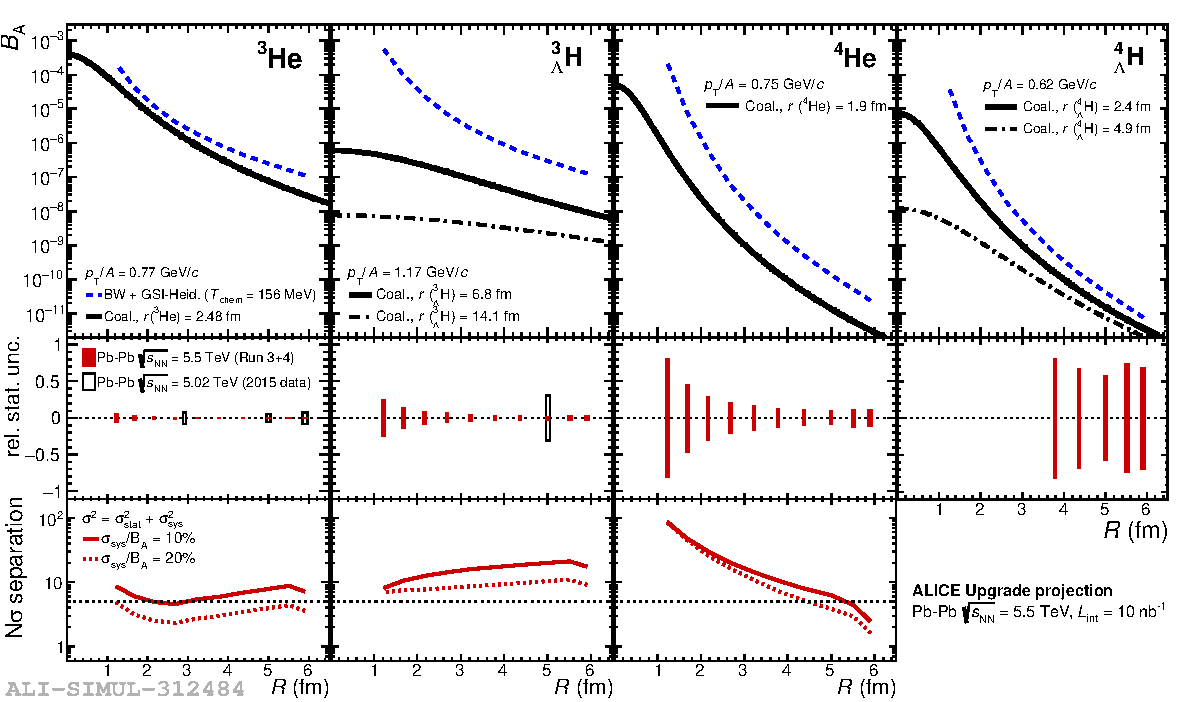
\includegraphics[width=\textwidth]{\main/lightflavour/figs/2018-10-23-2018-10-23-BAmodels_pseudoUnc.pdf}
\end{center}
\caption{
Top: comparison of predictions for the coalescence parameters for (hyper-)nuclei with \Anucl = 3, 4 from the Blast-Wave + GSI-Heidelberg thermal statistical model and coalescence as a function of the radius ($R$) of the particle emitting source. For each (hyper-)nucleus, the radius $r$ considered by the coalescence model is reported in the legend. For \hyp~(\hypfour), two values of the radius are considered: the lower value represents the average separation of the three (four) constituents, whereas the larger $r$ corresponds to the average separation between the $\Lambda$ and the deuteron (triton) core. See \cite{Bellini:2018epz} for full details on the models. Middle: projection of the relative statistical uncertainty achievable with a minimum bias \PbPb integrated luminosity of \Lint = 10 \nbInv and the upgraded ALICE detector (in red) compared to the relative statistical uncertainty of the Run 2 measurements (in black). Bottom: significance in the discrimination between the two models, assuming 10$\%$ and 20$\%$ systematic uncertainty in addition to the statistical uncertainty expected with \Lint = 10 \nbInv. For \hyp~and \hypfour, the coalescence predictions considered are  for $r = 6.8$ fm and $r = 2.4$ fm, respectively (corresponding to the black continuous lines in the top panels).}
\label{fig:BAmodels}
\end{figure}

\subsubsection{Light (anti-)(hyper-)nuclei observables in Runs 3 and 4}
\label{sec:hyper}

Measurements of (anti-)(hyper-)nuclei and exotic QCD bound states require large event samples collected with a minimum-bias trigger, as well as high tracking precision for the separation of secondary vertices and charged-hadron (light nucleus) identification. The upgraded ALICE detector after LS2 \cite{Abelevetal:2014dna, ALICE:2014qrd,alice-up-trg,Buncic:2015ari} fulfills these requirements, developing further the potential already explored in Runs 1 and 2.
The yields of (hyper-)nuclei (d,  \hethree, \hefour, \hyp, \hypfour, \hyphefour) and their anti-particles in \PbPb collisions at the LHC in Runs 3 and 4 have been estimated for measurements with ALICE. 
The detectable yield and significance for (anti-)(hyper-)nuclei have been estimated for 0--10\% central \PbPb collisions considering the acceptance and detection efficiency in the nominal magnetic field of the ALICE detector (B~=~0.5~T).
These projections are reported for anti-particles in Fig.~\ref{fig:yieldrun34} as a function of the minimum-bias integrated luminosity. The detectable particle and anti-particle yields are equivalent in the considered \pT\ range. 
All projections have been extracted in the $2 <\pT< 10~\gmom$ range, where the lower limit is given by the \pT\ down to which nuclei with \Anucl~$\geq$~3 can be reconstructed without ambiguity in ALICE. 
%During Run 3, ALICE plans to take data with a central-barrel low-field configuration (B~=~0.2~T) and to collect data in \PbPb collisions up to \Lint~=~3~\nbInv. 
In a scenario in which ALICE will take data with a central-barrel low-field configuration (B~=~0.2~T), it will be possible to extend the low-\pT\ limit for \mbox{(anti-)nuclei} identification down to 1~\gmom, increasing the expected number of detectable light \mbox{(anti-)(hyper-)nuclei} (by about 20$\%$ for \hethree). 
In Fig.~\ref{fig:yieldrun34}, the bands indicate the uncertainty on the yield (significance) associated with different model predictions:
the central line is obtained assuming statistical-thermal production with \Tchem~=~156~MeV~\cite{Andronic:2010qu}, the upper line is the yield (significance) assuming thermal production at \Tchem~=~158~MeV, and the lower one using for the yields the expectation from coalescence (see Sec.~\ref{sec:producionmodels}). 
The arrow represents the recorded luminosity at the end of the LHC Run 2. 
It has to be noted that for this study, the geometry of the ALICE Inner Tracking System (ITS) in Run 2 has been considered. 
The new geometry and acceptance of the upgraded ITS system \cite{Abelevetal:2014dna} are expected to increase the detection efficiency by up to 20\%.

\begin{figure}%[hbpt]
\begin{center}
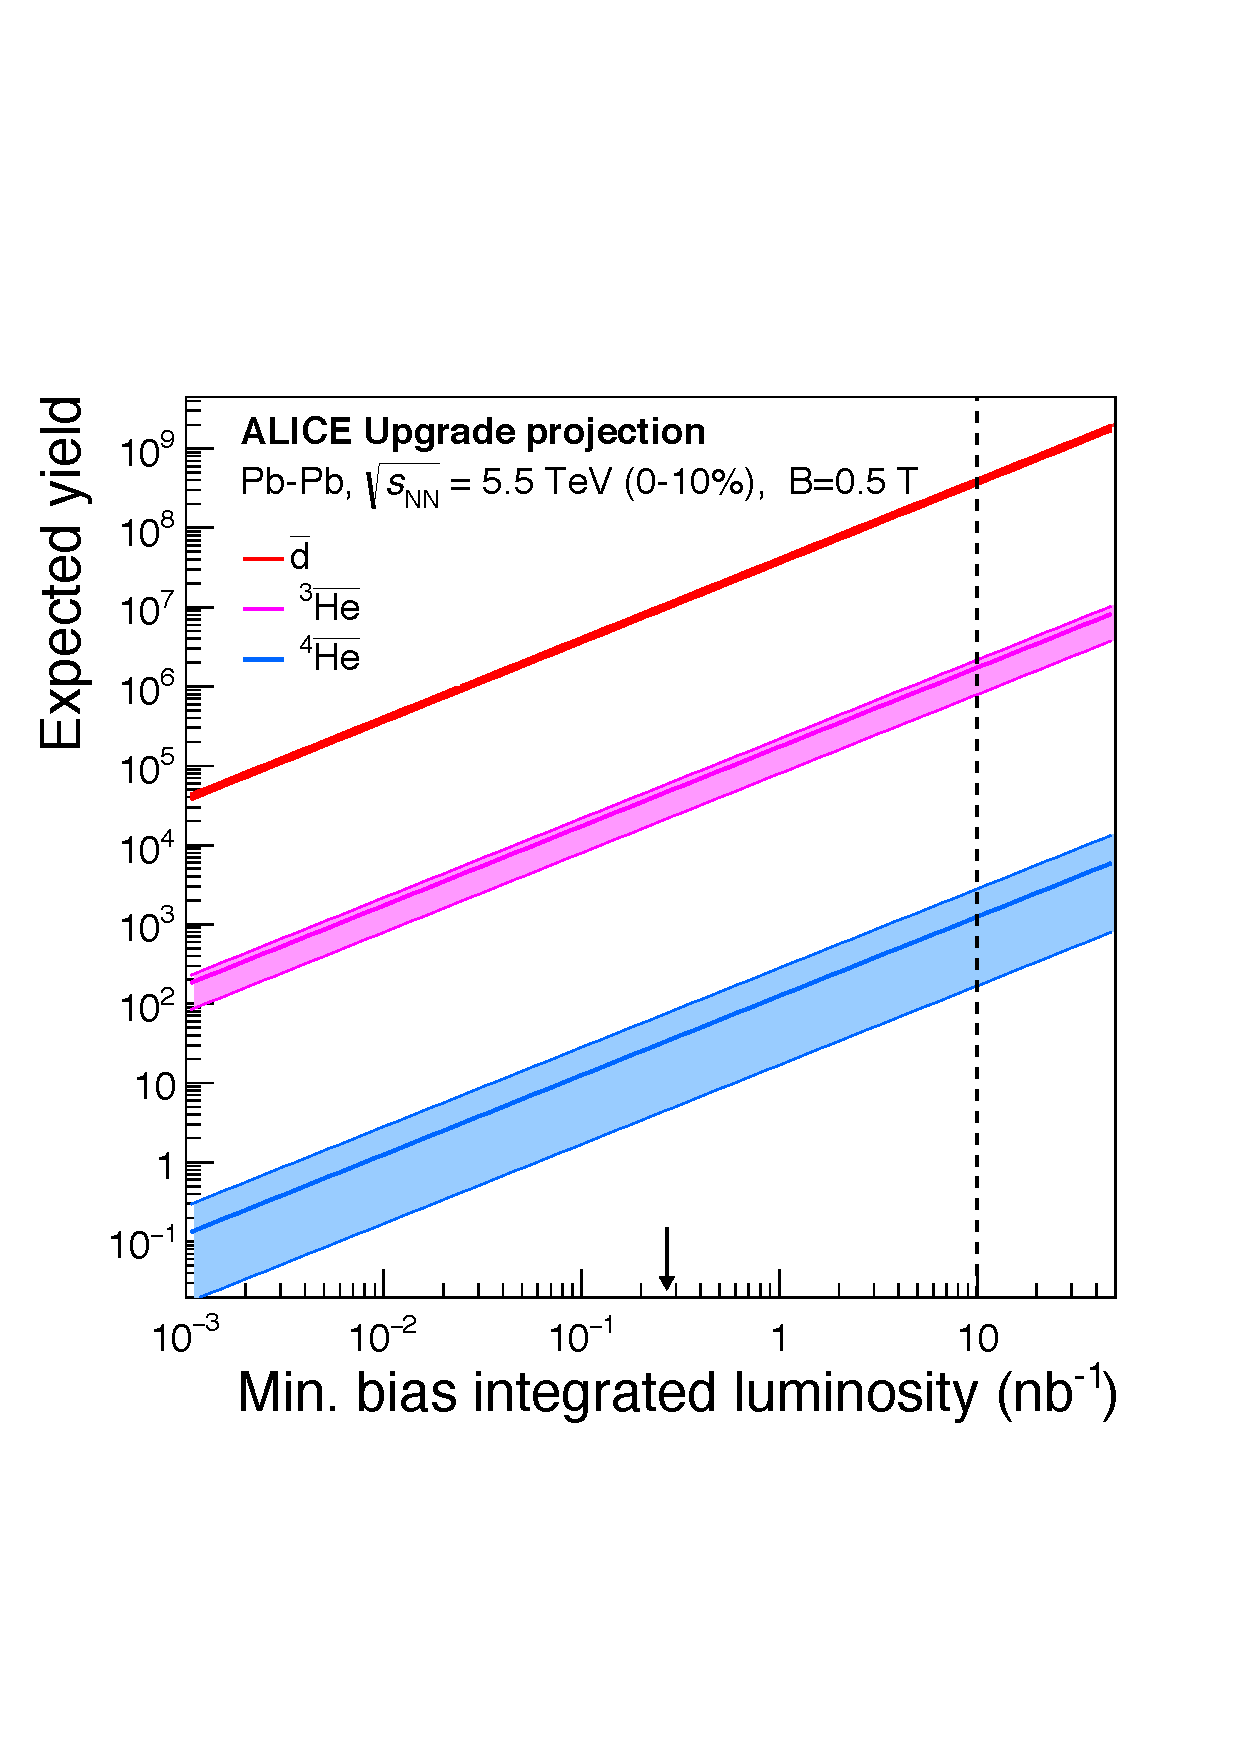
\includegraphics[width=0.49\textwidth]{\main/lightflavour/figs/nuclei_projection_10nb-1-presentITS.pdf}
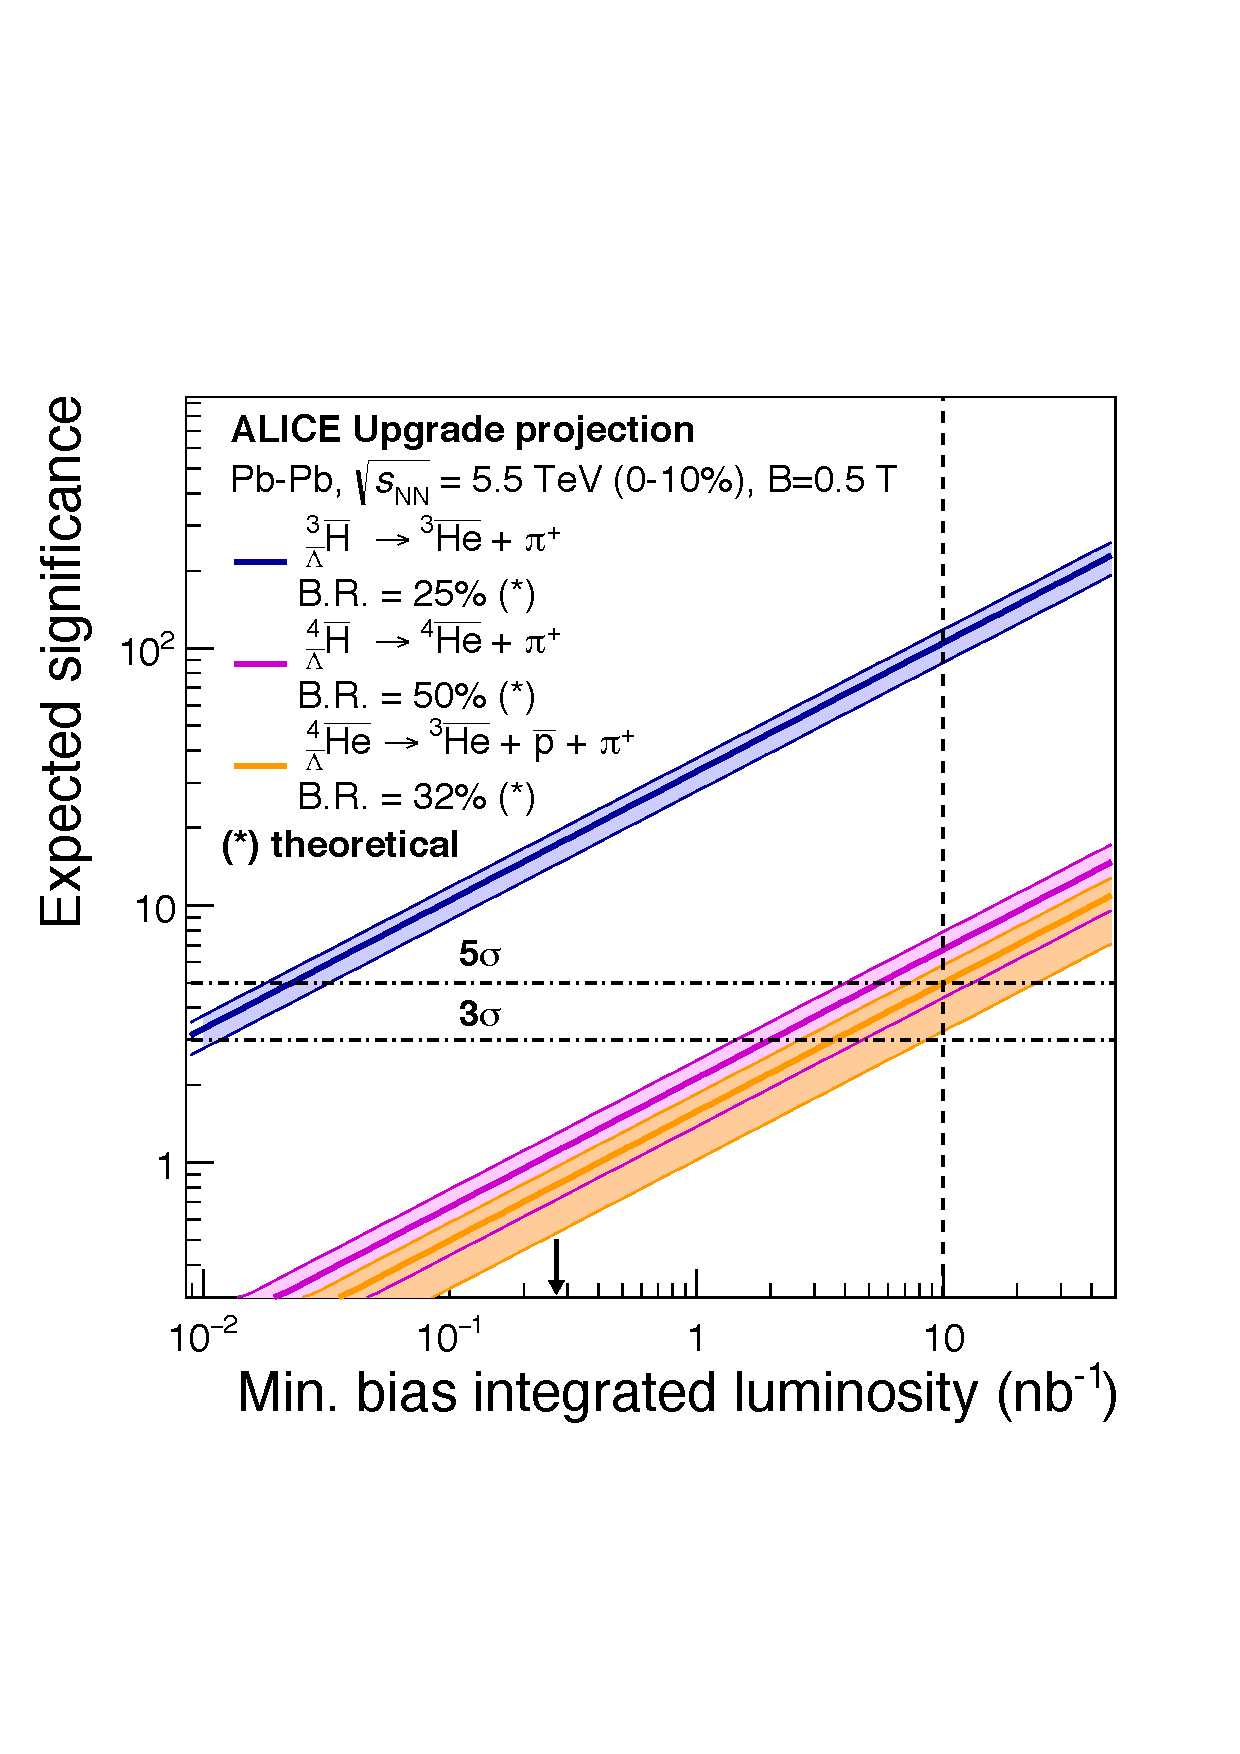
\includegraphics[width=0.49\textwidth]{\main/lightflavour/figs/hypernuclei_significance_10nb-1-presentITS.pdf}
\end{center}
\caption{\textcolor{red}{FIGURES TO BE RE-APPROVED BY ALICE AFTER SMALL UPDATE.}
Left: (raw) yield of anti-nuclei in the $2 <\pT< 10~\gmom$ interval, detectable in 0--10$\%$ central \PbPb collisions with the ALICE detector as a function of the minimum bias luminosity. 
Right: Projected significance of anti-hyper-nuclei measurements in central \PbPb collisions in Runs 3 and 4 with ALICE as a function of the integrated minimum-bias luminosity. In both panels, the arrow represents the minimum bias \PbPb luminosity anticipated for the end of Run 2. The dashed vertical line marks the projections with \Lint~=~10~\nbInv. The bands represents the uncertainty on model prediction for the yield (see text for details).
%and the black box in the right corner denotes a multiplicative factor representing the possible improvements related to use of the upgraded ALICE ITS.
}
\label{fig:yieldrun34}
\end{figure}

The expected yield per unit of rapidity at mid-rapidity are reported for \antid, \antihethree\ and \antihefour\ in left panel of Fig.~\ref{fig:yieldrun34}.
With \Lint~=~10~\nbInv recorded with the nominal magnetic field, a measurement of the elliptic flow ($v_2$) of \hethree~and \tritium~(and anti-nuclei) in \PbPb collisions will become feasible with ALICE with a statistical precision better than 5$\%$ in the $2-10~\gmom$ transverse momentum range in at least eight centrality intervals. 
Elliptic flow measurements for anti-nuclei provide a powerful independent test of coalescence scenarios as already demonstrated with deuterons \cite{Acharya:2017dmc} and might provide an indirect assessment of the neutron flow comparing the \hethree\ and \tritium\ results. 
%
In addition, the large data sample that will be collected for light anti-nuclei will lead to the first precise measurements of the mass of light anti-nuclei with \Anucl~=~3, by means of the Time-Of-Flight detector~\cite{Adam:2015pna}. 
This measurement will make it possible to test Charge Symmetry Breaking (CSB) in the anti-nuclei sector due to the differences in the up and down quark masses and due to electromagnetic effects \cite{Miller:1990ky}. 
The differences in \Anucl~=~3 systems are extensions of the neutron-proton difference. Although the mass difference for the lightest ``mirror pair'' with \Anucl~=~3 (i.e. \tritium,\hethree), is well known (at the level of O(eV)~\cite{Audi:2002rp}), no measurement has been performed in the anti-matter sector and will be accessible with \Lint~=~10~\nbInv. 

In the right panel of Fig.~\ref{fig:yieldrun34}, the expected significance of anti-hyper-nuclei measurements in central \PbPb collisions is reported as a function of the minimum bias integrated luminosity. 
For each species, the decay channels with the minimum number of charged particles in the final state and with the highest detection efficiency in ALICE have been considered for this study, as reported in the legend of Fig.~\ref{fig:yieldrun34}. 
The study of other decay channels, e.g. the three body decay of \hyp\ that has larger theoretical branching ratio with respect to the 2-body decay \cite{ Phys.Rev.C57}, but lower detection efficiency in ALICE, will be also carried out profiting from the large integrated luminosity.
Considering the thermal model predictions at \Tchem~=~156~MeV, the expected significance of \antihyp, \antihypfour\ and \antihehypfour\ at \Lint~=~10~\nbInv is 100, 7 and 5, respectively. 
The collected sample will enable very precise measurements of the production of \hyp\ and \antihyp\ and the first ever measurement of their elliptic flow as a function of \pT.
The discovery of \antihypfour\ and \antihehypfour\ will be in reach with \Lint~=~10~\nbInv at the end of Run 4.

\subsubsection{The hypertriton lifetime}
The experimental measurement of the $\Lambda$ separation energy of the \hyp, B$_{\Lambda}$ = 0.13 $\pm$ 0.05 (stat.) $\pm$ 0.04 (syst.) MeV \cite{davis20053}, led to the hypothesis that the lifetime of the hypertriton is equal to or only slightly below the free $\Lambda$ lifetime $\tau$($\Lambda$) = 263.2 $\pm$ 0.2 ps \cite{pdg:2018}.
Three different experimental techniques have been used to tackle this question: photographic emulsion, He bubble chambers, and counter experiments. The average for the emulsion experiments is 203$^{+40}_{-31}$ ps \cite{agnello:2016}, for the He bubble chambers is 193$^{+15}_{-13}$ ps \cite{agnello:2016}, and for the combination of both visualizing techniques is 193$^{+14}_{-13}$ ps \cite{agnello:2016}. The most recent results, 181 $^{+54}_{-39} \pm$ 33 ps and 142 $^{+24}_{-21} \pm$ 29 ps, have been obtained with the counter technique in heavy-ion collisions by the ALICE \cite{PhysLettB.754.360} and STAR \cite{PhysRevC.97.054909} experiments, respectively. This technique is currently the one with the highest precision (14-16$\%$) and the weighted average of heavy-ion experiments results is 185$^{+28}_{-23}$ ps \cite{agnello:2016}.
However, the few existing theoretical calculations point in the direction of the hypothesis mentioned at the beginning of this section. 
The first theoretical determination of $\tau$(\hyp) (by Dalitz and Rayet, \cite{NuovCim.A46}) ranged from 239.3 to 255.5 ps. More recent calculations from Congleton \cite{jphysg.18.339} and Kamada \cite{Phys.Rev.C57} estimated values of 232 ps and 256 ps, respectively. The deviation of the experimental results from the theoretical calculations and the free $\Lambda$ lifetime, by more than 2$\sigma$, is known as the ``hypertriton lifetime puzzle''.
 
With the expected integrated \PbPb luminosity at the end of the LHC Run 4, the statistical uncertainty on the lifetime will be reduced down to 1$\%$. 
%\todo{Stefano P: there are two values, you must specify what they refer to (hypertrion and anti-hypertriton? Run4 and Run3?)}
In parallel, a reduction of the systematic uncertainty ($\sim$ 10$\%$ in the most recent ALICE measurements), will be achieved with the upgraded ALICE ITS that will allow for a reduction of the uncertainty due to tracking and material budget. 
To improve even further down the control on the systematic uncertainty, a better understanding of the corrections for the absorption in the material will be crucial. 

\subsubsection{$\Sigma$-hypernuclei}
In addition to measurements of $\Lambda$-hypernuclei, also the search for $\Sigma$-hypernuclei is to be considered with the luminosities forseen for the LHC Runs 3 and 4. 
Theory calculations for the $\Sigma$NN system suggest the presence of a near-threshold narrow ($\sim$2 MeV wide) quasi-bound state in the \isospin~=~1 and \spinJ~=~1/2 configuration, where the possible isospin and spin states are 0, 1, 2 and 1/2, 3/2, respectively ~\cite{cite:SigmaTriton-theory}. 
Among $\Sigma$-hypernuclei, only the $_{\Sigma^0}^{4}\mathrm{He}$ bound state has been observed so far, using the ${^4}\mathrm{He}(K^-,\pi^-)$ reaction \cite{cite:SigmaTriton-data}.
When the $\Sigma^0$ hyperon is bound inside a nucleus, the electromagnetic decay is dominated by the conversion reaction $\Sigma^{0}\mathrm{N}\to\Lambda\mathrm{N}$, thus the partial width of electromagnetic decay is expected to be reduced substantially. 
However, for the \isospin~=~2 state the conversion reaction is not allowed and the electromagnetic decay becomes prominent.
%
Experimental searches for  $\Sigma$-hypertriton bound states will also profit from the \PbPb data-taking programme of the LHC Runs 3 and 4 to exploit the strong decay
$\sigmahyp~(\antisigmahyp)~\rightarrow~\Lambda~(\overline{\Lambda})~+~\mathrm{d}$
and the decay $\sigmahyp~(\antisigmahyp)~\rightarrow~\hyp~(\antihyp)~+~\gamma$
following a similar strategy to the detected electromagnetic decay of 
$\Sigma^{0}~(\overline{\Sigma}^{0})~\rightarrow~\Lambda~(\overline{\Lambda})~+~\gamma$~\cite{Borissov:2015ura}.
The signal of hypertriton can be reconstructed in ALICE as discussed in Sec.~\ref{sec:hyper}. The soft photon can be identified by exploiting the conversion into electron pairs in the detector material of the ITS and Time Projection Chamber ($X/X_0~\approx~9~\%$ considering the upgraded ITS and the TPC together), covering the pseudorapidity range $\vert\eta\vert~<~0.8$, over the full azimuth ($\Delta\varphi~=~2\pi$)~\cite{Abelev:2014ffa}.
Alternatively, the photon can be detected in the PHOS calorimeter, but with limited acceptance of $\Delta\varphi~=~100^{\mathrm{o}}$ and $\vert\eta\vert<~0.12$~\cite{Abelev:2014ffa}.
The search for $\Sigma$-hypernuclei via electromagnetic decay will be carried out in ALICE profiting from the expected detector performance and detection of about $10^5$ hypertriton candidates (see Fig.~\ref{fig:yieldrun34}) in 0--10\% central \PbPb collisions at \Lint~=~10~\nbInv.

\subsubsection{Exotic QCD bound states}
At LHC energies, potential QCD bound states that have more complex structures such as pentaquarks, tetraquarks, hadron molecules or dibaryon states could be produced.
In particular, the possibility to detect and measure f$_{0}$(980), N(1875), N$\Xi$, N$\Omega$ and N$\Lambda_c$ in heavy-ion collisions with the unprecedented statistics of the LHC Runs 3 and 4 programme has been investigated. The advanced capabilities of the ALICE experiment in terms of hadron identification, including topological reconstruction of weak decays, are particularly suited for these studies.

The per-event yields of these states (d$N$/d$y$)$_{\mathrm{th}}$) predicted by quark- and hadron-coalescence models \cite{Cho:2017dcy} and the statistical-thermal model \cite{Andronic:2017} are reported in Tab.~\ref{tab:yield}.

\begin{table}[!b]
\centering
\caption{Properties and yields of exotic states in 0--10\% central \PbPb collisions at $\sqrt{s_{\mathrm{NN}}} = 5.5$~TeV. Theoretical predictions of yields per event, (d$N$/d$y$)$_{\mathrm{th}}$, are given in three different scenarios: quark- and hadron-coalescence \cite{Cho:2017dcy}, and thermal model \cite{Andronic:2010qu}. $\mathrm{S_{raw}}$ represents the total detectable yield at the \PbPb luminosity of 10~\nbInv, taking into account the branching ratios (B.R.) of the decay channels considered and assuming the ALICE detector performance as in Run 2 \cite{Jacazio:2017dvy, Acharya:2018ckj}. For f$_0(980)$, a $\mathrm{K\overline{K}}$ state and a decay into $\mathrm{K\overline{K}}$ with B.R. = 10$^{-3}$ is assumed for hadron coalescence~$^{\dagger}$. A tetraquark state is assumed for quark coalescence and a decay into $\pi\pi$. The same decay channel is assumed for the thermal production case. Masses are from \cite{pdg:2017}.}
\label{tab:yield}
\resizebox{\textwidth}{!}{
\begin{tabular}{|c|c|c|c|c|c|c|}
\hline
 & Model & f$_{0}$(980)& N(1875)& N$\Xi$& N$\Omega$  & N$\Lambda_{c}$ \\
\hline
\hline
Structure & & $\mathrm{qq\bar{q}\bar{q}}$ or $\mathrm{K}\overline{\mathrm{K}}$ & hadron molecule & dibaryon & dibaryon  & dibaryon \\
 \hline
 &  q-coal. & 5.4 $\times$ 10$^{-2}$ &  - & - & 1.8 $\times$ 10$^{-3}$ & 1.5 $\times$ 10$^{-3}$ \\
 
$\big(\frac{\mathrm{d}N}{\mathrm{d}y}\big)_{\mathrm{th}}$ & h-coal. & 3.2 $^{\dagger}$       &  - & - & 1.6 $\times$ 10$^{-3}$ & 5   $\times$ 10$^{-3}$ \\

 & thermal &  10  & 3 $\times$ 10$^{-1}$ & 8.7 $\times$  10$^{-3}$ & 5.7 $\times$  10$^{-3}$ & 4 $\times$  10$^{-3}$ \\
\hline \hline
 Decay channel &
 & $\pi\pi$ / $\mathrm{K}\overline{\mathrm{K}}$ 
 & $\Sigma^{\ast}(\rightarrow \Lambda \pi)$K    
 & $\Xi\rightarrow \Lambda \pi$ & $\Omega \rightarrow \Lambda$K  
 & $\Lambda_{c}\rightarrow \pi$Kp + $\Lambda_{c}\rightarrow $K$^0_{\mathrm{S}}$p
\\

 B.R. ($\%$) & & dominant / seen$^{\dagger}$ & unknown (87) & 99.9 & 67.8 & 6.2 + 1.58 \\
Mass (MeV/$c^{2}$) & & 990 & 1850 -- 1920 & - & - & - \\
Width (MeV/$c^{2}$) & & 10 -- 100 & 120 -- 250 & - & - & - \\
\hline
\hline
					 & q-coal. & 1.8 $\times$ 10$^{8}$ & - & - & 6.2 $\times$ 10$^{4}$ & 1.5 $\times$ 10$^{4}$\\
 %$\big(\frac{\mathrm{d}N}{\mathrm{d}y}\big)_{\mathrm{exp}}$ & h-coal. & 6.4 $\times$ 10$^{6}$ $^{\dagger}$ & - & - & 5.5 $\times$ 10$^{4}$ & 5.1 $\times$ 10$^{4}$ \\
$\mathrm{S}_{\mathrm{raw}}$ & h-coal. & 6.4 $\times$ 10$^{6}$ $^{\dagger}$ & - & - & 5.5 $\times$ 10$^{4}$ & 5.1 $\times$ 10$^{4}$ \\
  					& thermal & 3.6 $\times$ 10$^{10}$ & 5.5 $\times$ 10$^{7}$& 6.7 $\times$ 10$^5$ & 1.9 $\times$ 10$^{5}$ & 4.1 $\times$ 10$^{4}$\\

\hline
               & q-coal. & 130-3.5 & - & - & - & - \\
\significance & h-coal. & - & - & - & - & - \\
 			   & thermal & 2600-70 & 520-360 & - & - & - \\

\hline
\end{tabular}
}
\end{table}

The total number of signals (S$_{\mathrm{raw}}$) detectable in ALICE with a minimum bias \PbPb integrated luminosity of 10~\nbInv have been estimated assuming the same detector performance as in Run 2 \cite{Jacazio:2017dvy, Acharya:2018ckj}. 
The significance is defined as \significance, where S and B are the integrals of the signal and background distributions, respectively, in a $\pm~3~\sigma$ window centered at the nominal mass from \cite{pdg:2018}. 
$\sigma$ is $\Gamma/2.35$, where $\Gamma$ is the resonance width taken from \cite{pdg:2018}. 
The significance for f$_0$(980) and N(1835) was extracted assuming a combinatorial background in the invariant mass range under study. 
Such combinatorics was computed based on particle species that can populate the invariant mass distribution, 
making use of the corresponding momentum distribution as measured in ALICE in Run 2 (e.g. individual primary charged pions paired as candidates for the f$_{0}$(980)$~\rightarrow~\pi^{+}+\pi^{-}$ channel)
%The expected background was computed from the momentum distributions of the decay products as measured in ALICE in Run 2. 
%In particular, the momentum components of the decay products were extracted randomly according to the measured transverse momentum distribution of each candidate (considered as a probability distribution) 
and assuming a uniform distribution in $\varphi$ and $\eta$ \footnote{An additional factor is introduced if the decay particle is reconstructed via invariant mass, since the candidate may belong also to the background.}.
The resulting significance is reported in the last row of Tab.~\ref{tab:yield} for the most pessimistic scenario, in which production occurs via quark coalescence, and the most optimistic scenario, corresponding to thermal production. 


Measurements of f$_{0}$(980) and N(1875) will be feasible in Runs 3 and 4 and will shed light on the highly-debated nature of the states (hadrons or hadronic molecules). 
In particular, the N(1875) can be considered a molecular bound state and at the same time the strange partner of the recently discovered pentaquark P$_{c}$ \cite{He:2017aps}. 
Because the structure of exotic states is related to the fundamental properties of Quantum Chromodynamics (QCD), their observation can provide new insights on the properties of QCD at finite temperature and density, for instance that tetraquark condensation may lead to a second chiral phase transition \cite{Cho:2017dcy}.
Several possible states have been studied and predictions are available on the expected yields at LHC energies \cite{Cho:2017dcy}. Among the possible dibaryon bound states, the N$\Omega$, N$\Xi$ and N$\Lambda_c$ look promising in terms of detection feasibility. Their detection and baryon-baryon correlations will be useful for hyperon correlation studies, providing new insights into the baryon-baryon attractive potential as well as upper limits on the formation of such bound states in central heavy-ion collisions.

